\documentclass[10pt,UKenglish, leqno, xcolor = dvipsnames]{beamer}

\usetheme{UiB}

% Font choice:
\usefonttheme{default}

\usepackage{cite}
\usepackage{subfig}
\usepackage{amsmath, amsthm, mathtools, color, setspace}
\usepackage{fancyhdr, braket, etoolbox,booktabs,multirow}
\usepackage{xfrac, lmodern, ifsym, bm, multicol, booktabs, pdflscape}
\usepackage[utf8]{inputenx} % For æ, ø, å
\usepackage{csquotes}       % Quotation marks
\usepackage{microtype}      % Improved typography
\usepackage{amssymb}        % Mathematical symbols
\usepackage{mathtools,physics,centernot,tensor}      % Mathematical symbols
\usepackage[absolute, overlay]{textpos} % Arbitrary placement
\setlength{\TPHorizModule}{\paperwidth} % Textpos units
\setlength{\TPVertModule}{\paperheight} % Textpos units
\usepackage[dvipsnames]{xcolor}

\usepackage{calrsfs}
\DeclareMathAlphabet{\pazocal}{OMS}{zplm}{m}{n}

\usepackage{tikz}
\usetikzlibrary{tikzmark,calc,overlay-beamer-styles,arrows,shapes}  % Overlay effects for TikZ
\newenvironment{proenv}{\only{\setbeamercolor{local structure}{fg=RoyalBlue}}}{}
\newenvironment{conenv}{\only{\setbeamercolor{local structure}{fg=Maroon}}}{}
\newenvironment{bibbianoenv}{\only{\setbeamercolor{local structure}{fg=Green}}}{}
\DeclarePairedDelimiter{\insieme}{\{}{\}}
\newcommand{\numberset}{\mathbb}
\newcommand{\alg}{\mathfrak}
\newcommand{\Z}{\numberset{Z}}
\newcommand{\R}{\numberset{R}}
\newcommand{\N}{\numberset{N}}
\newcommand{\C}{\numberset{C}}
\newcommand{\A}{\alpha}

\usepackage{stackengine}
\def\tanslant{.25}
\newcommand\hatsrm[2][2]{\ensurestackMath{%
		\ifnum#1>1%
		\stackengine{-4pt}{\hatsrm[\numexpr#1-1\relax]{#2}}{%
			\scriptstyle\char'136}{O}{c}{F}{T}{S}%
		\else%
		\stackengine{-3pt}{#2}{\scriptstyle\char'136}{O}{c}{F}{T}{S}%
		\fi%
}}
\newcommand\hatsit[2][2]{\ensurestackMath{%
		\sbox0{$#2$}%
		\ifnum#1>1%
		\stackengine{-4pt}{\hatsit[\numexpr#1-1\relax]{#2}}{%
			\kern\tanslant\ht0\scriptstyle\char'136}{O}{c}{F}{T}{S}%
		\else%
		\stackengine{-3pt}{#2}{\kern\tanslant\ht0\scriptstyle\char'136}%
		{O}{c}{F}{T}{S}%
		\fi%
}}

\usetikzlibrary{chains, positioning, shapes.symbols}
\tikzset{start/.style = {signal, 
						fill=#1,
						draw=white,
						font=\tiny,
						text=white,
						inner sep=2pt,
						signal pointer angle=90,
		 				on chain},
						cont/.style = {start=#1, signal from=west}
		}

\usepackage{tcolorbox}
\newtcolorbox{box1}[1]{colback=white!5!white,colframe=green!60!white,fonttitle=\bfseries,title=#1}
\newtcolorbox{box2}[1]{colback=white!5!white,colframe=red!60!gray,fonttitle=\bfseries,title=#1}

\author{Pietro Daniele}
\title{\large Search for new resonances in the 100 to 195 GeV diphoton invariant mass range using 140 fb$^{-1}$ of $pp$ collisions collected at $\sqrt{s}$=13 TeV with the ATLAS detector}

\begin{document}
	\tikzstyle{na} = [baseline=-.5ex]
	\tikzstyle{every picture}+=[remember picture]
	
	\begin{frame}{Standard Model (SM)}
		\vfill
		The Standard Model of particle physics is a quantum field theory:
		\begin{itemize}
			\item based on SU(2)$_L\otimes$U(1)$_Y\otimes$SU(3)$_C$\\ gauge symmetry
			\item explains the basic building blocks of\\ matter interactions
			\item classifies all the subatomic known\\ particles
			\item predicted new particles:
			\begin{itemize}
				\item gluon
				\item top ($t$) and charm ($c$) quarks
				\item $W$ and $Z$ bosons %$\leftarrow$ \textit{mass-less}
				\item Higgs boson
				\begin{itemize}
					\item gives mass to the other particles
					\item discovered by the ATLAS and CMS\\ experiments in July 2012 
					\item $m_H$ = 125.09$\pm$0.24 GeV (Run1)
				\end{itemize}
			\end{itemize}
		\end{itemize}
		
		%$W$ and $Z$ bosons discovered in 1983
		%$
		%\begin{cases}
		%		m_W = 80\ GeV\\
		%		m_Z = 91\ GeV\\
		%	\end{cases}
		%	$\\
		%	$\Rightarrow$ the introduction of $W,Z$ mass terms in the SM Lagrangian would break the local gauge invariance of the theory\\ 
		%	\begin{center}
	%		$\Rightarrow$ \textit{Spontaneous Symmetry Breaking}\\
	%		$\Rightarrow$ \textbf{Higgs Boson}
	%	\end{center}
		\vfill
		\begin{textblock}{1.}(0.525,.275)
			\includegraphics[width=.45\textwidth]{../thesis_images/SM.jpeg}
		\end{textblock}
	\end{frame}

	\begin{frame}{SM limitations}
		\vfill
		SM is not the final theory of nature:
		\begin{itemize}
			\item no dark matter candidate  
			\item no explanation for the matter-antimatter\\ asymmetry 
		\end{itemize}
		\begin{textblock}{1.}(.6,.26)
			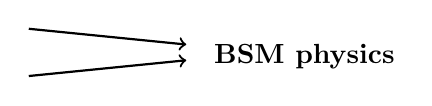
\begin{tikzpicture}
				\draw[-to,thick] (0,.8) -- (2,0.6);
				\draw[-to,thick] (0,.2) -- (2,0.4);
				\path (3.5,0.45) node {\textbf{BSM physics}};
			\end{tikzpicture}
		\end{textblock}
		\vspace{1cm}
		Higgs field:
		\begin{itemize}
			\item a complex doublet under SU(2)$_L$ symmetry group
			\item could be extended $\Rightarrow$ larger scalar sectors:
			\begin{itemize}
				\item additional structures $\Rightarrow$ \textbf{NEW BOSONS}
				\item new theory
				\begin{itemize}
					\item 2HDM $\leftarrow$ \textit{bottom-up} approach
					\item SUSY $\leftarrow$ \textit{top-down} approach
				\end{itemize}
			\end{itemize} 
		\end{itemize}
		\vfill
	\end{frame}

	\begin{frame}{$H\to\gamma\gamma$ channel}
		\vspace{.2cm}
		$H\to\gamma\gamma$ is a channel that could be used for the new spin-0 resonances search
		\begin{itemize}
			\item Non resonant background
			\vspace{1.5cm}
			\item final state kinematic fully\\ reconstructed
			\item Excellent invariant mass\\ resolution (1-2 GeV)
			\item the signal appears a peak over\\ the expected background
		\end{itemize}
		\vfill
		\begin{textblock}{1.}(0.5,.425)
			\includegraphics[width=.5\textwidth]{../thesis_images/higgs_boson_plot.png}
		\end{textblock}
		\begin{textblock}{1.}(.475,.24)
			\begin{itemize}
				\footnotesize
				\item Irr $\to$ QCD di-photon production
				\vspace{.2cm}
				\item Red $\to$ ($\gamma$,jet), (jet,jet) with jet\\ misidentification (\textit{fake rate})
			\end{itemize}
		\end{textblock}
		\begin{textblock}{1.}(.25,.225)
			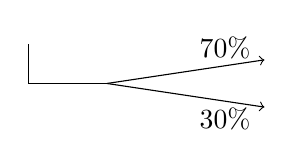
\begin{tikzpicture}
				\draw[-] (-1,0.5) -- (-1,0);
				\draw[-] (-1,0) -- (0,0);
				\draw[-to] (0,0) -- (2.,0.3);
				\path (1.5,0.45) node {70\%};
				\draw[-to] (0,0) -- (2.,-0.3);
				\path (1.5,-0.45) node {30\%};
			\end{tikzpicture}
		\end{textblock}
		\begin{textblock}{1.}(.185,.65)
			\begin{tikzpicture}
				\draw[-to,black!30] (0,0) -- (7,0);
			\end{tikzpicture}
		\end{textblock}
	\end{frame}
		
	\begin{frame}{New spin-0 resonances analysis}
		\vfill
		\begin{center}
			BSM physics $\Rightarrow$ New spin-0 resonances search
		\end{center}
		\begin{itemize}
			\item \textbf{Channel}: $H \to \gamma\gamma$
			\item \textbf{Aim}: 
			\begin{itemize}
				\item find an excess of events over \\the expected background by\\ fitting the $m_{\gamma\gamma}$ spectrum
				\item $[100,195]$ GeV $m_{\gamma\gamma}$ range
			\end{itemize}
			
			\item \textbf{Signal}:
			\begin{itemize}
				\item $X \to \gamma\gamma$ 
				\item a function of the resonance\\ mass $m_X$
				\item small SM assumptions
			\end{itemize}
			\item \textbf{Background}
			\begin{itemize}
				\item Non resonant background
				\item SM Higgs boson background
			\end{itemize}
			\item \textbf{Results}: combined maximum likelihood fit
		\end{itemize}
		\vfill 
		\begin{textblock}{1}(.45,.3)
			\includegraphics[width=.6\textwidth]{../thesis_images/MC_sample_140.pdf}
		\end{textblock}
	\end{frame}
	
	\begin{frame}{Signal model SM independence}
		\vfill
		New physics search:\\
		$\Rightarrow$  An analysis as much independent as possible from assumptions based on Standard Model
		\begin{itemize}
			\item the intrinsic amplitude of the Higgs boson resonance ($m_H=125$ GeV $\to$ $\sigma$ = 4 MeV) is negligible compared to the resolution 
			\item the SM Higgs production modes are: \textit{ggF} (80\%), \textit{VBF}(10\%) \dots
			\item only \textit{ggF} is considered for the signal model creation
			\item other production modes included as a signal yield systematic uncertainty $\sigma^{prod\ modes}$
		\end{itemize}
		\vspace{.8cm}
		\resizebox{.5\textwidth}{1.3cm}{
			\begin{box1}{Advantages}
				\begin{itemize}
					\item small assumptions on the production modes for the new resonances
					\item include and parameterise the ignorance of the relative importance of different production modes for additional scalar Higgs bosons searches.
				\end{itemize}
			\end{box1}
		}\resizebox{.5\textwidth}{1.3cm}{
			\begin{box2}{Disadvantages}
				\begin{itemize}
					\item $\sigma^{prod\ modes}$ increases in the more granular categorisation\\
					$\Rightarrow$ the analysis performances decrease
					\item No Higgs discovery Run1 categorisation
				\end{itemize}
			\end{box2}
		}
		\vfill
		\begin{textblock}{1}(0.,.85)
			\begin{figure}
				\resizebox{\textwidth}{!}{
					\begin{tikzpicture}[
						node distance = 0mm,
						start chain = going right,
						]
						\node[start=gray!20!white, scale=1] {Categories};
						\node[cont=uibblue!80!black,   scale=1] {Sig model};
						\node[cont=gray!20!white,   scale=1] {Bkg model};
						\node[cont=gray!20!white,   scale=1.1] {HSM model};
						\node[cont=gray!20!white,   scale=1] {Syst uncs};
						\node[cont=gray!20!white,   scale=1] {Exp results};
					\end{tikzpicture}		
				}
			\end{figure}
		\end{textblock}
	\end{frame}

	\begin{frame}{LHC}
		\vfill
		\begin{itemize}
			\item The \textit{Large Hadron Collider} (LHC) \\is a protons and heavy ions collider\\ installed in the 27 km long LEP \\tunnel
			\item Run2 $pp$ collisions $\sqrt{s} = 13$ TeV
			\item Four leading experiments installed\\ in the four $pp$ interaction points:
			\begin{itemize}
				\item \textbf{ATLAS}
				\item CMS
				\item LHCb
				\item ALICE
			\end{itemize}
		\end{itemize}
		\vfill
		\begin{textblock}{1.}(0.5,.2)
			\includegraphics[width=.5\textwidth]{../thesis_images/CERN_complex.png}
		\end{textblock}
	\end{frame}
	
	\begin{frame}{ATLAS}
		\vfill
		The ATLAS experiment:
		\begin{itemize}
			\item a multi purpose detector
			\item forward-backward symmetric detector with a $\sim4\pi$ angular coverage
			\item composed of several layers:
			\begin{itemize}
				\item Inner Detector (ID)
				\item Calorimetric system
				\item Muon Spectrometer
			\end{itemize}
			\item Magnetic field:
			\begin{itemize}
				\item a solenoid
				\item a barrel toroid and\\ two end-cap toroids
			\end{itemize}
			\item Trigger system
			\begin{itemize}
				\item 40 MHz $\to$ 1 kHz
			\end{itemize}
			
		\end{itemize}
		\vfill
		\begin{textblock}{1.}(0.375,.45)
			\includegraphics[width=.575\textwidth]{../thesis_images/ATLAS.png}
		\end{textblock}
	\end{frame}
	
	\begin{frame}{Events Selection}
		\vfill
		$H \to \gamma\gamma$ channel: \textbf{Event selected}
		\begin{itemize}
			\item Event selection aimed at reducing the $\gamma$-jet and di-jet bkg and at finding two good-quality photonss
			\item $m_{\gamma\gamma}\ \epsilon\ [100,195]$ GeV mass range
			\item two photons:
			\begin{itemize}
				\item $|\eta|<2.37$
				\item identified
				\item isolation
				\item $p_T^{\gamma_i}/m_{\gamma\gamma}$ (>0.3, >0.25)
				%\item $p_T^{\gamma_1}/m_{\gamma\gamma}$ > 0.3 
				%\item $p_T^{\gamma_2}/m_{\gamma\gamma}$ > 0.25
			\end{itemize}
		\end{itemize}
		\vspace{.3cm}
		\centering
		$\Downarrow$
		\begin{enumerate}\centering
			\item Categorisation
			\item Signal model
			\item Non-resonant background model
			\item SM Higgs boson background model
			\item Systematic uncertainties
			\item Expected results
		\end{enumerate}
		\vfill
	\end{frame}
	
	\begin{frame}{Categorisation}
		\vfill
		\begin{itemize}
			\item The events are classified into\\ mutually exclusive categories
			\item Designed to enhance the analysis\\ sensitivity
			\begin{itemize}
				\item maximise the signal and\\ bkg ratio $\frac{S}{B}$
				\item minimise the systematic\\ uncertainties
			\end{itemize}
			\item three categorisations tested and\\ compared:
			\begin{itemize}
				\item \texttt{Inclusive}, \texttt{catConvEta}, \texttt{catConv}
				\item $\gamma$ conversion status 
				\item $\eta$ position cuts ($|\eta|<2.37$)
				\begin{itemize}
					\item central region $|\eta|<0.75$
					\item trans region $ \eta \epsilon [1.3,1.75]$
					\item no central and trans regions
				\end{itemize}
			\end{itemize}
		\end{itemize}
		\begin{textblock}{1}(.5,.15)
			\includegraphics[width=.5\textwidth]{../thesis_images/inclusive_tree.pdf}\\
			\includegraphics[width=.5\textwidth]{../thesis_images/catConvEta_tree.pdf}\\
			\includegraphics[width=.5\textwidth]{../thesis_images/catConv_tree.pdf}\\	
		\end{textblock}	
		\vfill
		\begin{textblock}{1.}(.2,.2125)
			\begin{tikzpicture}
				\draw[-to,black!30] (0,-4) -- (4,0);
			\end{tikzpicture}
		\end{textblock}
		\begin{textblock}{1.}(.35,.425)
			\begin{tikzpicture}
				\draw[-to,black!30] (0,-2) -- (2,0);
			\end{tikzpicture}
		\end{textblock}
		\begin{textblock}{1.}(.45,.67)
			\begin{tikzpicture}
				\draw[-to,black!30] (0,0) -- (0,-0.1)
				node[below] {} -- (.5,-.1);
			\end{tikzpicture}
		\end{textblock}
		\begin{textblock}{1}(0.,.85)
			\begin{figure}
				\resizebox{\textwidth}{!}{
					\begin{tikzpicture}[
						node distance = 0mm,
						start chain = going right,
						]
						\node[start=uibblue!80!black, scale=1] {Categories};
						\node[cont=gray!20!white,   scale=1] {Sig model};
						\node[cont=gray!20!white,   scale=1] {Bkg model};
						\node[cont=gray!20!white,   scale=1.1] {HSM model};
						\node[cont=gray!20!white,   scale=1] {Syst uncs};
						\node[cont=gray!20!white,   scale=1] {Exp results};
					\end{tikzpicture}		
				}
			\end{figure}
		\end{textblock}
	\end{frame}

	\begin{frame}{Signal model}
		\vfill
		For each category:
		\begin{itemize}
			\item \textbf{Function form}: \textit{Double-Sided Crystal\\ Ball} (DSCB):
			\begin{itemize}
				\item a gaussian core + power-law tails
				\item 6 parameters ($\mu, \sigma, a_{1,2}, p_{1,2}$)
			\end{itemize}
			\item \textbf{Samples}: \textit{ggF} MC samples with four\\ different resonance mass $m_X$ (110, 125,\\ 130 and 140 GeV)
			\item \textbf{Fit}: a simultaneous DSCB fit:
			\begin{itemize}
				\item $[100,195]$ GeV $m_{\gamma\gamma}$ range
				\item DSCB parameters $\propto$ $m_X$:\\
				$par(m_X) = A^{par} + B^{par}\cdot m_X$
				\item $A$ and $B$ params fixed after fit\\
			\end{itemize}
		\end{itemize}
		\vspace{.5cm}
		\vfill
		\begin{textblock}{1}(.575,.125)
			\includegraphics[width=.45\textwidth]{../thesis_images/PowhegPy8_NNLOPS_ggH125_catConvEta_no_fit.pdf}\\
			\includegraphics[width=.45\textwidth]{../thesis_images/sigma_postfit.pdf}\\
		\end{textblock}	
		\begin{textblock}{1}(0.,.85)
			\begin{figure}
				\resizebox{\textwidth}{!}{
					\begin{tikzpicture}[
						node distance = 0mm,
						start chain = going right,
						]
						\node[start=gray!20!white, scale=1] {Categories};
						\node[cont=uibblue!80!black,   scale=1] {Sig model};
						\node[cont=gray!20!white,   scale=1] {Bkg model};
						\node[cont=gray!20!white,   scale=1.1] {HSM model};
						\node[cont=gray!20!white,   scale=1] {Syst uncs};
						\node[cont=gray!20!white,   scale=1] {Exp results};
					\end{tikzpicture}		
				}
			\end{figure}
		\end{textblock}
	\end{frame}

	\begin{frame}{Signal yield($m_X$)}
		\vspace{.5cm}
		In each category $i$, the signal yield is expressed as:
		$$
		N^i(m_X) = \sigma_{ggF}(m_X) \cdot Br_{\gamma\gamma}(m_X) \cdot \mathcal{L}_{Run2} \cdot A_X(m_X)  \cdot C_X^i(m_X)
		$$
		\vspace{.3cm}\\
		\textit{Fiducial} volume:
		\begin{itemize}
			\item region characterized by kinematics selections at the MC generation level
			\item \textit{Fiducial} events $\to$ fiducial criteria mimic the selection criteria		
		\end{itemize}
		\begin{center}
			\begin{table}[tbp]
				\centering
				\resizebox{8.5cm}{!}{
					\small
					\begin{tabular}{llcc}
						\toprule[1.5pt]
						Parameter									& Name						& Reconstruction Level	& Truth Level		\\
						\midrule
						$|\eta^{\gamma_i}|$							& $\eta$ cut				& $<2.37$ 				& $<2.37$			\\
						$p_T^{\gamma_1}/m_{\gamma\gamma}$			& Scalar relative $p_T$ cut & > 0.3					& > 0.3    			\\
						$p_T^{\gamma_2}/m_{\gamma\gamma}$			& Scalar relative $p_T$ cut & > 0.25				& > 0.25			\\
						$E_{T}^{cone20\ \gamma_i}/p_T^{\gamma_i}$ 	& Isolation cut 			& < 0.065				& < 0.065 			\\
						$p_{T}^{cone20\ \gamma_i}/p_T^{\gamma_i}$ 	& Isolation cut 			& < 0.05				& 		 			\\
						\bottomrule[1.5pt]
					\end{tabular}
				}
			\end{table}
		\end{center}
		\begin{textblock}{1}(0.,.85)
			\begin{figure}
				\resizebox{\textwidth}{!}{
					\begin{tikzpicture}[
						node distance = 0mm,
						start chain = going right,
						]
						\node[start=gray!20!white, scale=1] {Categories};
						\node[cont=uibblue!80!black,   scale=1] {Sig model};
						\node[cont=gray!20!white,   scale=1] {Bkg model};
						\node[cont=gray!20!white,   scale=1.1] {HSM model};
						\node[cont=gray!20!white,   scale=1] {Syst uncs};
						\node[cont=gray!20!white,   scale=1] {Exp results};
					\end{tikzpicture}		
				}
			\end{figure}
		\end{textblock}
	\end{frame}
	
	\begin{frame}{Non-resonant background}
		\vfill
		For each category:
		\begin{itemize}
			\item modelled using MC samples
			\item \textbf{Functional form}:\\ $f^i_{bkg}(m_{\gamma\gamma},N_{bkg}^i,a^i,b^i) = N_{bkg}^i\cdot\exp^{(a^i\cdot m_{\gamma\gamma}+b^i\cdot m_{\gamma\gamma}^2)}$
			\begin{itemize}
				\item $N^{i}_{bkg}$, $a_i$, $bi$ are free parameters
			\end{itemize} 
			\item \textbf{Sample}: di-photon MC samples
			\item \textbf{Fit}: \textit{exp(poly2)} fit:
			\begin{itemize}
				%\item blind search $\to$ [110,170] GeV\\ $m_X$ range
				\item fit $\to$  [100,195] GeV $m_{\gamma\gamma}$ range
			\end{itemize}
			\item the functional form, chosen using\\ MC samples, will applied to data
		\end{itemize}
		\vspace{.5cm}
		\vfill
		\begin{textblock}{1}(.495,.4)
			\includegraphics[width=.55\textwidth]{../thesis_images/bkg_100_195GeV_fit_catConvEta_no_prova.pdf}\\	
		\end{textblock}
		\begin{textblock}{1}(0.,.85)
			\begin{figure}
				\resizebox{\textwidth}{!}{
					\begin{tikzpicture}[
						node distance = 0mm,
						start chain = going right,
						]
						\node[start=gray!20!white, scale=1] {Categories};
						\node[cont=gray!20!white,   scale=1] {Sig model};
						\node[cont=uibblue!80!black,   scale=1] {Bkg model};
						\node[cont=gray!20!white,   scale=1.1] {HSM model};
						\node[cont=gray!20!white,   scale=1] {Syst uncs};
						\node[cont=gray!20!white,   scale=1] {Exp results};
					\end{tikzpicture}		
				}
			\end{figure}
		\end{textblock}
	\end{frame}
	
	\begin{frame}{Higgs Standard Model background}
		\vfill
		For each category:
		\begin{itemize}
			\item \textbf{Function form}: \textit{Double-Sided Crystal\\ Ball} (DSCB):
			\begin{itemize}
				\item a gaussian core + power-law tails
				\item 6 parameters ($\mu, \sigma, a_{1,2}, p_{1,2}$)
			\end{itemize}
			\item \textbf{Samples}: all SM Higgs 125 GeV\\ production modes MC sample
			\item \textbf{Fit}: a single DSCB fit:
			\begin{itemize}
				\item DSCB parameters fixed after the fit
				\item $[100,195]$ GeV $m_{\gamma\gamma}$ range
				\item yield set from SM predictions
			\end{itemize}
		\end{itemize}
		\vspace{.75cm}
		\vfill
		\begin{textblock}{1}(.575,.3)
			\includegraphics[width=.45\textwidth]{../thesis_images/bkg/HSM_fit_catConvEta_no.pdf}\\	
		\end{textblock}
		\begin{textblock}{1}(0.,.85)
			\begin{figure}
				\resizebox{\textwidth}{!}{
					\begin{tikzpicture}[
						node distance = 0mm,
						start chain = going right,
						]
						\node[start=gray!20!white, scale=1] {Categories};
						\node[cont=gray!20!white,   scale=1] {Sig model};
						\node[cont=gray!20!white,   scale=1] {Bkg model};
						\node[cont=uibblue!80!black,   scale=1.1] {HSM model};
						\node[cont=gray!20!white,   scale=1] {Syst uncs};
						\node[cont=gray!20!white,   scale=1] {Exp results};
					\end{tikzpicture}		
				}
			\end{figure}
		\end{textblock}
	\end{frame}

	\begin{frame}{Systematic Uncertainties}
		\vfill
		Systematic uncertainties
		\begin{itemize}
			\item arise from experimental sources
			\item estimated for each category
			\item  are included into the likelihood model of the measurement as nuisance parameters
			\item divided into two different groups:
		\end{itemize}
		\vspace{.5cm}
		\begin{enumerate}\centering
			\item shape systematic uncertainties
			\item yield systematic uncertainties
		\end{enumerate}
		\vfill
		\begin{textblock}{1}(0.,.85)
			\begin{figure}
				\resizebox{\textwidth}{!}{
					\begin{tikzpicture}[
						node distance = 0mm,
						start chain = going right,
						]
						\node[start=gray!20!white, scale=1] {Categories};
						\node[cont=gray!20!white,   scale=1] {Sig model};
						\node[cont=gray!20!white,   scale=1] {Bkg model};
						\node[cont=gray!20!white,   scale=1.1] {HSM model};
						\node[cont=uibblue!80!black,   scale=1] {Syst uncs};
						\node[cont=gray!20!white,   scale=1] {Exp results};
					\end{tikzpicture}		
				}
			\end{figure}
		\end{textblock}
	\end{frame}

	\begin{frame}{Shape systematic uncertainties}
		\vfill
		Shape systematic uncertainties $\to$ the\\ modelling of $m_{\gamma\gamma}$ distribution:
		\begin{itemize}
			\item photon energy scale uncertainties:
			\begin{itemize}
				\item affect the peak position ($\mu^{DSCB}$)
				%\item $\delta\mu_c(\pm1\sigma)=\frac{<m_{\gamma\gamma}>_i(\pm1\sigma)}{<m_{\gamma\gamma}>_i}-1$
				\item impact of less than 0.5\%
				%\item only on signal model
			\end{itemize}
			\item photon energy resolution uncertainties
			\begin{itemize}
				\item affect the Gaussian width ($\sigma^{DSCB}$)
				%\item $\delta\sigma_c(\pm1\sigma)=\frac{IQR_i(\pm1\sigma)}{IQR_i}-1$
				\item impact of less than 12\%
				%\item on signal and HSM models
			\end{itemize}
			\item LHC Higgs mass uncertainty
			\begin{itemize}
				\item affect the peak position ($\mu^{DSCB}$)
				\item impact of 0.2\%
				\item only on HSM model
			\end{itemize}
		\end{itemize}
		\vspace{.2cm}
		\vfill
		\begin{textblock}{1}(.575,.125)
			\includegraphics[width=.4\textwidth]{../thesis_images/Syst/var_shape_scale_catConvEta_no.pdf}\\
			\includegraphics[width=.4\textwidth]{../thesis_images/Syst/var_shape_res_catConvEta_no.pdf}\\	
		\end{textblock}	
		\begin{textblock}{1}(0.,.85)
			\begin{figure}
				\resizebox{\textwidth}{!}{
					\begin{tikzpicture}[
						node distance = 0mm,
						start chain = going right,
						]
						\node[start=gray!20!white, scale=1] {Categories};
						\node[cont=gray!20!white,   scale=1] {Sig model};
						\node[cont=gray!20!white,   scale=1] {Bkg model};
						\node[cont=gray!20!white,   scale=1.1] {HSM model};
						\node[cont=uibblue!80!black,   scale=1] {Syst uncs};
						\node[cont=gray!20!white,   scale=1] {Exp results};
					\end{tikzpicture}		
				}
			\end{figure}
		\end{textblock}
	\end{frame}

	\begin{frame}{Yield systematic uncertainties}
		\vspace{.2cm}
		Yield systematic uncertainties $\to$ the expected signal and HSM yields
		\begin{itemize}
			\item the $\gamma$ energy scale and resolution uncertainties on the selection efficiency
			\item the $\gamma$ identification and\\ isolation efficiencies
			\item the efficiency of the\\ diphoton trigger
			\item  the modelling of pile-up\\ in the simulation\\
			\vspace{.1cm}
		\end{itemize}
		$\Rightarrow$ an impact of less than 2\%
		\begin{textblock}{1}(.375,.25)
			\includegraphics[width=.65\textwidth]{../thesis_images/Syst/var_catConvEta_no_sig_fid.pdf}\\	
		\end{textblock}
		\begin{textblock}{1}(0.,.85)
			\begin{figure}
				\resizebox{\textwidth}{!}{
					\begin{tikzpicture}[
						node distance = 0mm,
						start chain = going right,
						]
						\node[start=gray!20!white, scale=1] {Categories};
						\node[cont=gray!20!white,   scale=1] {Sig model};
						\node[cont=gray!20!white,   scale=1] {Bkg model};
						\node[cont=gray!20!white,   scale=1.1] {HSM model};
						\node[cont=uibblue!80!black,   scale=1] {Syst uncs};
						\node[cont=gray!20!white,   scale=1] {Exp results};
					\end{tikzpicture}		
				}
			\end{figure}
		\end{textblock}
	\end{frame}

	\begin{frame}{Yield systematic uncertainties}
		\vfill
		Yield systematic uncertainties $\to$ the expected signal and HSM yields\\
		The production mode dependence $\sigma^{prod\ modes}$
		\begin{itemize}
			\item on signal model
			\item For each category $C_X^{prod}$\\ parametrised as functions\\ of $m_X$
			\item $\sigma^{prod\ modes}$ is maximum of \\linear fits difference by\\ varying prod modes\\ and resonance mass
		\end{itemize}
		\vspace{.5cm}
		\vfill
		\begin{textblock}{1}(.4,.325)
			\includegraphics[width=.65\textwidth]{../thesis_images/Signal/cx_all_prod_catConvEta_no.pdf}\\	
		\end{textblock}	
		
		\begin{textblock}{1}(0.,.85)
			\begin{figure}
				\resizebox{\textwidth}{!}{
					\begin{tikzpicture}[
						node distance = 0mm,
						start chain = going right,
						]
						\node[start=gray!20!white, scale=1] {Categories};
						\node[cont=gray!20!white,   scale=1] {Sig model};
						\node[cont=gray!20!white,   scale=1] {Bkg model};
						\node[cont=gray!20!white,   scale=1.1] {HSM model};
						\node[cont=uibblue!80!black,   scale=1] {Syst uncs};
						\node[cont=gray!20!white,   scale=1] {Exp results};
					\end{tikzpicture}		
				}
			\end{figure}
		\end{textblock}
	\end{frame}

	\begin{frame}{Combined maximum likelihood fit}
		\vfill
		Selected events, different categorisations, models and systematic uncertainties are used as building blocks for a combined maximum likelihood fit:
		\begin{itemize}
			\item a method of estimating the parameters which maximise an assumed probability distribution ($\pazocal{L}$ likelihood), given data.
			\item the systematic uncertainties and the non-resonant bkg model parameter are inserted in the fit as Nuisance Parameters (\textbf{NPs})
			\item $\sigma^{fid}$ is the \textbf{POI} of the fit which is performed simultaneously over every category of a specific categorisation for different $m_X$ values
			\item the maximum likelihood fit estimates:
			\begin{itemize}
				\item the POI $\sigma^{fid}$  $\leftarrow$ free
				\item NPs
				\begin{itemize}
					\item Systematic Uncertainties $\leftarrow$ constrained 
					\item Non-res bkg parameters $\leftarrow$ free
				\end{itemize}
			\end{itemize}
		\end{itemize}
		\vspace{.2cm}
		\vfill
		\begin{textblock}{1}(0.,.85)
			\begin{figure}
				\resizebox{\textwidth}{!}{
					\begin{tikzpicture}[
						node distance = 0mm,
						start chain = going right,
						]
						\node[start=gray!20!white, scale=1] {Categories};
						\node[cont=gray!20!white,   scale=1] {Sig model};
						\node[cont=gray!20!white,   scale=1] {Bkg model};
						\node[cont=gray!20!white,   scale=1.1] {HSM model};
						\node[cont=gray!20!white,   scale=1] {Syst uncs};
						\node[cont=uibblue!80!black,   scale=1] {Exp results};
					\end{tikzpicture}		
				}
			\end{figure}
		\end{textblock}
	\end{frame}
	
	\begin{frame}{Expected results}
		\vspace{.4cm}
		$\Longrightarrow$ a combined maximum likelihood fit in all the categories is performed
		\begin{itemize}
			\item investigating the presence of a signal by computing the compatibility of the MC template with\\ the background\\ only hypothesis $p_0$
			%\item assessing limits, in a fiducial region, on the\\ x-s in case no excess of signal is observed.
		\end{itemize}	
		\begin{textblock}{1}(.3,.275)	
			\includegraphics[width=.725\textwidth]{../thesis_images/p0_catConvEta_pres.pdf}\\
			%\includegraphics[width=.45\textwidth]{../thesis_images/plot_AsimovData_0_ggHyy_MC_no_catConvEta_syst_HSM_fid_nom_gaus.pdf}	
		\end{textblock}
		\begin{textblock}{1}(0.,.85)
			\begin{figure}
				\resizebox{\textwidth}{!}{
					\begin{tikzpicture}[
						node distance = 0mm,
						start chain = going right,
						]
						\node[start=gray!20!white, scale=1] {Categories};
						\node[cont=gray!20!white,   scale=1] {Sig model};
						\node[cont=gray!20!white,   scale=1] {Bkg model};
						\node[cont=gray!20!white,   scale=1.1] {HSM model};
						\node[cont=gray!20!white,   scale=1] {Syst uncs};
						\node[cont=uibblue!80!black,   scale=1] {Exp results};
					\end{tikzpicture}		
				}
			\end{figure}
		\end{textblock}
	\end{frame}
	
	\begin{frame}{Expected results}
		\vspace{.4cm}
		$\Longrightarrow$ a combined maximum likelihood fit in all the categories is performed
		\begin{itemize}
			%\item investigating the presence of a signal by\\ computing the compatibility of the MC\\ template with the background-only\\ hypothesis $p_0$
			\item assessing limits, in a fiducial region, on the x-s in case no excess of signal is observed.
		\end{itemize}		
		\begin{textblock}{1}(.3,.275)
			%\includegraphics[width=.45\textwidth]{../thesis_images/p0_no_catConvEta.pdf}\\
			\includegraphics[width=.725\textwidth]{../thesis_images/xs_fid_AsimovData_0_ggHyy_MC_catConvEta_syst_HSM_fid_nom_gaus_pres.pdf}	
		\end{textblock}
		\begin{textblock}{1}(0.,.85)
			\begin{figure}
				\resizebox{\textwidth}{!}{
					\begin{tikzpicture}[
						node distance = 0mm,
						start chain = going right,
						]
						\node[start=gray!20!white, scale=1] {Categories};
						\node[cont=gray!20!white,   scale=1] {Sig model};
						\node[cont=gray!20!white,   scale=1] {Bkg model};
						\node[cont=gray!20!white,   scale=1.1] {HSM model};
						\node[cont=gray!20!white,   scale=1] {Syst uncs};
						\node[cont=uibblue!80!black,   scale=1] {Exp results};
					\end{tikzpicture}		
				}
			\end{figure}
		\end{textblock}
	\end{frame}

	\begin{frame}{Expected results}
		\vfill
		\textbf{Without} systematic uncertainties improvement\\ compared to \texttt{Inclusive} category
		\begin{itemize}
			\item discovery potential
			\begin{itemize}
				\item \texttt{catConvEta} $\to$ $\sim$6.3\%
				\item \texttt{catConv} $\to$ $\sim$1.2\%
			\end{itemize}
			\item limits setting
			\begin{itemize}
				\item \texttt{catConvEta} $\to$ $\sim$7.6\%
				\item \texttt{catConv} $\to$ $\sim$2.4\%
			\end{itemize}
		\end{itemize}
		\textbf{With} systematic uncertainties improvement\\ compared to \texttt{Inclusive} category
		\begin{itemize}
			\item limits setting
			\begin{itemize}
				\item \texttt{catConvEta}
				\begin{itemize}
					\item always positive improvement
					\item maximum value 4.2\% at $m_X$=170 GeV
				\end{itemize}
				\item \texttt{catConv}
				\begin{itemize}
					\item not always positive improvement\\
					$\Rightarrow$ should be discarded
				\end{itemize}
			\end{itemize}
		\end{itemize}
		\vspace{.5cm}
		\vfill
		\begin{textblock}{1}(.5825,.1)	
			\includegraphics[width=.45\textwidth]{../thesis_images/p0_exp_imp.pdf}\\
			\includegraphics[width=.45\textwidth]{../thesis_images/imp_nom_gaus.pdf}	
		\end{textblock}
		\begin{textblock}{1}(0.,.85)
			\begin{figure}
				\resizebox{\textwidth}{!}{
					\begin{tikzpicture}[
						node distance = 0mm,
						start chain = going right,
						]
						\node[start=gray!20!white, scale=1] {Categories};
						\node[cont=gray!20!white,   scale=1] {Sig model};
						\node[cont=gray!20!white,   scale=1] {Bkg model};
						\node[cont=gray!20!white,   scale=1.1] {HSM model};
						\node[cont=gray!20!white,   scale=1] {Syst uncs};
						\node[cont=uibblue!80!black,   scale=1] {Exp results};
					\end{tikzpicture}		
				}
			\end{figure}
		\end{textblock}
	\end{frame}

	\begin{frame}{Conclusions}
		\vfill
		\begin{itemize}
			\item The potential of search for new resonances in [100,195] GeV $m_{\gamma\gamma}$ range has been investigated
			\item The best categorisation obtained from the trade-off between performances and SM independence is \texttt{catConvEta}:
			\begin{itemize}
				\item a signal significance ranging from few $\sigma$ to $\sim$12$\sigma$ can be achieved in the search for new spin-0 resonance, assuming the SM mass dependence of the cross-section
				\item the excluded fiducial cross-section for a signal ranges from $\sim$3.4 pb to $\sim$34.6 pb depending on the new resonance mass.
			\end{itemize}
			\item The analysis is still blind so no results based on data have been shown
			\item The results presented in this thesis represent the first step towards the unblinding.
		\end{itemize} 
		\vfill
	\end{frame}

	%%%%%%%%% Backup %%%%%%%%%
	\section{Backup}
	\SectionPage
		
		\begin{frame}{Spontaneous Symmetry Breaking}
			With the \textit{Higgs mechanism} and the \textit{Spontaneous Symmetry Breaking} is possible to introduce a gauge invariant mass term of the $W,Z$ gauge boson
		\end{frame}
	
		\begin{frame}{ATLAS coordinate system}
			\vspace{.2cm}
			ATLAS coordinate system
			\begin{itemize}
				\item origin at the nominal interaction point
				\item $z$-axis along the beam axis, ($x$-$y$) transverse plane
				\item azimuthal angle $\phi$
				\item polar angle $\theta$
				\item pseudorapidity $\eta$ = -$\ln(\tan(\frac{\theta}{2}))$
			\end{itemize}
			\begin{textblock}{1}(.275,.5)
				%\includegraphics[width=.45\textwidth]{../thesis_images/p0_no_catConvEta.pdf}\\
				\includegraphics[width=.75\textwidth]{../thesis_images/atlas_eta_coord.png}	
			\end{textblock}
			
		\end{frame}
	
		\begin{frame}{2HDM}
			\vfill
			Two Higgs Doublet Model (2HDM)
			\begin{itemize}
				\item there are two Higgs fields, $\phi_1$ and $\phi_2$, both of which are complex doublets.
				\item the Higgs potential
				\begin{equation*}\begin{split}
						V =\ & m^2_{11}\phi_1^{\dagger}\phi_1 + m^2_{22}\phi_2^{\dagger}\phi_2 - [m^2_{12}\phi_1^{\dagger}\phi_2 + h.c.] +
						\lambda_1(\phi_1^{\dagger}\phi_1)^2 + \lambda_2(\phi_2^{\dagger}\phi_2)^2\\ & + \lambda_3(\phi_1^{\dagger}\phi_1)(\phi_2^{\dagger}\phi_2) + \lambda_4(\phi_1^{\dagger}\phi_2)(\phi_2^{\dagger}\phi_1) + [\lambda_5(\phi_1^{\dagger}\phi_2)^2 + h.c.]
				\end{split}\end{equation*}
				\item  Five physical states: two CP-even Higgs bosons $h$ (HSM boson) and $H$ (scalars), a $CP$-odd Higgs boson $A $(pseudoscalar), and two charged Higgs bosons $H^{\pm}$
				\item The most general 2HDM contains 14 free parameters.
			\end{itemize}
			\vfill
		\end{frame}
	
		\begin{frame}{SUSY}
			\vspace{.2cm}
			Super Symmetry (SUSY)
			\begin{itemize}
				\item is an extension of the Standard Model that aims to fill some of the gap
				\item predicts a partner particle for each particle in the Standard Model
				\begin{itemize}
					\item fermion$^{SM}$ $\to$ boson$^{SUSY}$
					\item boson$^{SM}$ $\to$ fermion$^{SUSY}$
				\end{itemize}
				\item Motivation
				\begin{enumerate}
					\item SUSY allows unification of forces
					\item SUSY cancels the SM divergences
					\item Lightest SUSY particle is a candidate for DM
					\item SUSY provides a theoretical route to implement gravity in SM
				\end{enumerate}
			\end{itemize}
			\begin{textblock}{1}(.275,.65)
				%\includegraphics[width=.45\textwidth]{../thesis_images/p0_no_catConvEta.pdf}\\
				\includegraphics[width=.5\textwidth]{../thesis_images/susy.jpg}	
			\end{textblock}
		\end{frame}
	
		\begin{frame}{Event reconstruction}
			\vfill
			The events reconstruction mainly exploits informations coming from
			\begin{itemize}
				\item the electromagnetic calorimeter (clusters)
				\item the Inner Detector (ID) systems (tracks)
			\end{itemize}
			
			Using these informations
			\begin{itemize}
				\item a converted photon is a cluster matched to either two tracks forming a conversion vertex, or one track without hits in the innermost pixel layer;
				\item an unconverted photon is a cluster matched to neither an electron track nor a conversion vertex.
			\end{itemize}
			\vfill
		\end{frame}
	
		\begin{frame}{Event reconstruction}
			\vfill
			\centering
			\includegraphics[width=.8\textwidth]{../thesis_images/alg_flow.png}	
			\vfill
		\end{frame}
	
		\begin{frame}{Event reconstruction}
			\vfill	
			The reconstruction of photons with $|\eta| < 2.37$ proceeds following these steps
			\begin{enumerate}
				\item the algorithm first prepares the tracks and clusters it will use
				\begin{itemize}
					\item it selects clusters of energy deposits measured in topologically connected EM and hadronic calorimeter cells, denoted topo-clusters
				\end{itemize}
				\item these clusters are matched to ID tracks
				\item the algorithm also builds conversion vertices and matches them to the selected topo-clusters
				\item the electron and photon supercluster-building steps then run separately
				\item the supercluster-building algorithm matches tracks to the electron superclusters and conversion vertices to the photon superclusters
				\item The electron and photon objects to be used for analyses are then built, their energies are calibrated, and discriminating variables used to separate electrons or photons from background are added.
			\end{enumerate}
			\vfill
		\end{frame}
	
		\begin{frame}{Monte Carlo samples}
			\vfill
			\centering
			\begin{table}[tbp]
				\centering
				\begin{tabular}{lcccc}
					\toprule[1.5pt]
					Process					& Generator						& Showering			& PDF set				& $\sigma^{125 GeV}$ [pb]		\\
					\midrule
					\textit{ggF}			& \texttt{Powheg NNLOPS}		& \texttt{Pythia}	& \texttt{PDF4LHC15}	& 48.5				\\
					\textit{VBF}			& \texttt{Powheg}				& \texttt{Pythia}	& \texttt{NNPDF3.0}		& 3.78				\\
					\textit{W$^+$H}			& \texttt{Powheg}				& \texttt{Pythia}	& \texttt{PDF4LHC15}	& 1.37				\\
					\textit{W$^-$H}			& \texttt{Powheg}				& \texttt{Pythia}	& \texttt{PDF4LHC15}	& 1.37				\\
					\textit{qq$\to$ZH}		& \texttt{Powheg}				& \texttt{Pythia}	& \texttt{PDF4LHC15}	& 0.76				\\
					\textit{gg$\to$ZH}		& \texttt{Powheg}				& \texttt{Pythia}	& \texttt{PDF4LHC15}	& 0.12				\\
					\textit{t$\bar{t}$H}	& \texttt{Powheg}				& \texttt{Pythia}	& \texttt{PDF4LHC15}	& 0.51				\\
					\textit{b$\bar{b}$H}	& \texttt{Powheg}				& \texttt{Pythia}	& \texttt{PDF4LHC15}	& 0.49				\\
					\textit{tHbj}			& \texttt{MadGraph5\_aMC@NLO}	& \texttt{Pythia}	& \texttt{PDF4LHC15}	& 0.074				\\
					\textit{tHW}			& \texttt{MadGraph5\_aMC@NLO}	& \texttt{Pythia}	& \texttt{PDF4LHC15}	& 0.015				\\
					\midrule
					\textit{$\gamma\gamma^{QCD}$} &  \texttt{Sherpa}		& \texttt{Sherpa}	& \texttt{NNPDF3.0}		&					\\
					\bottomrule[1.5pt]	
				\end{tabular}
			\end{table}	
			\vfill
		\end{frame}
	
		\begin{frame}{Asimov dataset}
			\vspace{.2cm}
			The Asimov dataset is an artificial dataset, used for estimating the sensitivity of the analysis under certain hypotheses
			\begin{itemize}
				\item it is a single representative dataset, where all the statistical fluctuations are suppressed
				\item It is designed starting from a given model, and it is constructed such that when one uses it to evaluate the estimators for all parameters, one obtains the true parameter values
			\end{itemize}
			\begin{textblock}{1}(.375,.425)
				\includegraphics[width=.65\textwidth]{../thesis_images/HSM_prova.pdf}
			\end{textblock}
		\end{frame}
	
		\begin{frame}{SM Higgs production modes}
			\vfill
			\centering
			\begin{figure}
				\centering
				\subfloat[]{\includegraphics[width=.3\textwidth]{../thesis_images/ggF.png}}
				\subfloat[]{\includegraphics[width=.3\textwidth]{../thesis_images/VBF.png}}					
				\caption{Examples of leading-order Feynman diagrams for Higgs boson production via the (a) \textit{ggF} and (b) \textit{VBF} production processes.}
			\end{figure}
			\vfill
		\end{frame}

		\begin{frame}{SM Higgs production modes}
			\vfill
			\begin{figure}
				\centering
				\subfloat[]{\includegraphics[width=.3\textwidth]{../thesis_images/qqVH.png}}
				\hspace{.2cm}
				\subfloat[]{\includegraphics[width=.3\textwidth]{../thesis_images/ggZH1.png}}
				\hspace{.2cm}				
				\subfloat[]{\includegraphics[width=.3\textwidth]{../thesis_images/ggZH2.png}}	
				\caption{Examples of leading-order Feynman diagrams for Higgs boson production via the (a) $qq\to VH$ and (b,c) $gg\to ZH$ production processes.}
			\end{figure}
			\vfill
		\end{frame}
	
		\begin{frame}{SM Higgs production modes}
			\vfill
			\centering
			\begin{figure}
				\centering
				\subfloat[]{\includegraphics[width=.3\textwidth]{../thesis_images/qqH.png}}
				\hspace{.2cm}
				\subfloat[]{\includegraphics[width=.3\textwidth]{../thesis_images/ggH1.png}}
				\hspace{.2cm}				
				\subfloat[]{\includegraphics[width=.3\textwidth]{../thesis_images/ggH2.png}}
				\caption{Examples of leading-order Feynman diagrams for Higgs boson production via the $qq/gg\to ttH$ and $qq/gg\to bbH$ processes.}
			\end{figure}
			\vfill
		\end{frame}

		\begin{frame}{SM Higgs production modes}
			\vfill
			\begin{figure}
				\centering
				\subfloat[]{\includegraphics[width=.225\textwidth]{../thesis_images/tHq1.png}}
				\hspace{.1cm}
				\subfloat[]{\includegraphics[width=.225\textwidth]{../thesis_images/tHq2.png}}
				\hspace{.1cm}				
				\subfloat[]{\includegraphics[width=.225\textwidth]{../thesis_images/tHW1.png}}
				\hspace{.1cm}
				\subfloat[]{\includegraphics[width=.225\textwidth]{../thesis_images/tHW2.png}}
				\caption{Examples of leading-order Feynman diagrams for Higgs boson production in association with a single top quark via the (a,b) $tHq$ and (c,d) $tHW$ production processes.}
			\end{figure}
			\vfill
		\end{frame}

		\begin{frame}{SM Higgs production modes x-s}
			\vfill
			\begin{figure}
				\centering
				\includegraphics[width=.6\textwidth]{../thesis_images/higgs_xs.png}
				\caption{The production cross section of the Higgs boson as a function of the Higgs mass at the LHC.}
			\end{figure}
			\vfill
		\end{frame}
		
		\begin{frame}{Run1 Categorisation}
			\vspace{.5cm}
			The Run1 mass categorisation used for the 125 GeV Standard Model Higgs boson discovery is based on
			\begin{itemize}
				\item $\gamma$ conversion status
				\item $\eta$ position
				\item $p_{Tt_{\gamma\gamma}}$ momentum 
			\end{itemize}
			\vspace{.2cm}
			$\Rightarrow$ It can not be used in this analysis since\\ it has an enormous impact on the model\\ dependence.		
			\begin{textblock}{1}(.25,.225)
				\begin{table}[htbp]
					\centering
					\begin{tabular}{lc}
						\toprule[1.5pt]
						Category			& $\sigma^{prod\ modes}$	\\
						\midrule
						Inclusive			& 0.044				\\
						\midrule
						catMass\_Run1\_1 	& 0.440				\\
						catMass\_Run1\_2 	& 5.972				\\
						catMass\_Run1\_3 	& 0.512				\\
						catMass\_Run1\_4 	& 4.116				\\
						catMass\_Run1\_5 	& 0.144				\\
						catMass\_Run1\_6 	& 0.438				\\
						catMass\_Run1\_7 	& 5.788				\\
						catMass\_Run1\_8 	& 0.533				\\
						catMass\_Run1\_9 	& 4.008				\\
						catMass\_Run1\_10 	& 0.153				\\
						\bottomrule[1.5pt]
					\end{tabular}
				\end{table}
			\end{textblock}

			\begin{textblock}{1}(0.,.85)
				\begin{figure}
					\resizebox{\textwidth}{!}{
						\begin{tikzpicture}[
							node distance = 0mm,
							start chain = going right,
							]
							\node[start=uibblue!80!black, scale=1] {Categories};
							\node[cont=gray!20!white,   scale=1] {Sig model};
							\node[cont=gray!20!white,   scale=1] {Bkg model};
							\node[cont=gray!20!white,   scale=1.1] {HSM model};
							\node[cont=gray!20!white,   scale=1] {Syst uncs};
							\node[cont=gray!20!white,   scale=1] {Exp results};
						\end{tikzpicture}		
					}
				\end{figure}
			\end{textblock}
		\end{frame}
		
		\begin{frame}{DSCB parameters}
			\vspace{.2cm}
			DSCB parameter for the signal model are inserted in the analysis as a linear function of $m_X$ :
			\begin{enumerate}
				\item a single DSCB fit is applied on every \textit{ggF} MC sample with different $m_X$ (110, 125, 130 and 140 GeV)
				\item the 4 $\sigma^{DSCB}$ are fitted using a linear fit
				\item the coefficients (A,B) of\\ this preliminary fit are used\\ as input for the \\simultaneous DSCB fit
				\item the A and B coefficients after\\ the simultaneous DSCB fit\\ are inserted in the analysis\\ fixed
			\end{enumerate}
			$\Rightarrow$ Analysis sensitive to new\\ spin-0 resonances
			\begin{textblock}{1}(.425,.38)
				\includegraphics[width=.6\textwidth]{../thesis_images/sigma_comp.pdf}
			\end{textblock}
			\begin{textblock}{1}(0.,.85)
				\begin{figure}
					\resizebox{\textwidth}{!}{
						\begin{tikzpicture}[
							node distance = 0mm,
							start chain = going right,
							]
							\node[start=gray!20!white, scale=1] {Categories};
							\node[cont=uibblue!80!black,   scale=1] {Sig model};
							\node[cont=gray!20!white,   scale=1] {Bkg model};
							\node[cont=gray!20!white,   scale=1.1] {HSM model};
							\node[cont=gray!20!white,   scale=1] {Syst uncs};
							\node[cont=gray!20!white,   scale=1] {Exp results};
						\end{tikzpicture}		
					}
				\end{figure}
			\end{textblock}
		\end{frame}
		
		\begin{frame}{Signal yield($m_X$)}
			\vfill
			In each category $i$, the signal yield is expressed as:
			$$
			N^i(m_X) = \sigma_{ggF}(m_X) \cdot A_X(m_X) \cdot Br_{\gamma\gamma}(m_X) \cdot \mathcal{L}_{Run2} \cdot C_X^i(m_X)
			$$
			\begin{center}
				\includegraphics[width=.35\textwidth]{../thesis_images/x_section_fit.pdf}
				\includegraphics[width=.35\textwidth]{../thesis_images/ax_isFiducialMedium_linear_fit.pdf}\\
				\includegraphics[width=.35\textwidth]{../thesis_images/br_fit.pdf}			
				\includegraphics[width=.35\textwidth]{../thesis_images/cx_fit_catConvEta_no.pdf}
			\end{center}
			\vfill
			\begin{textblock}{1}(0.,.85)
				\begin{figure}
					\resizebox{\textwidth}{!}{
						\begin{tikzpicture}[
							node distance = 0mm,
							start chain = going right,
							]
							\node[start=gray!20!white, scale=1] {Categories};
							\node[cont=uibblue!80!black,   scale=1] {Sig model};
							\node[cont=gray!20!white,   scale=1] {Bkg model};
							\node[cont=gray!20!white,   scale=1.1] {HSM model};
							\node[cont=gray!20!white,   scale=1] {Syst uncs};
							\node[cont=gray!20!white,   scale=1] {Exp results};
						\end{tikzpicture}		
					}
				\end{figure}
			\end{textblock}
		\end{frame}
	
		\begin{frame}{Spurious signal}
			\vfill
			Spurious signal
			\begin{itemize}
				\item a non-zero signal amplitude obtained when fitting Sig+Bkg model to data that is known to be signal-free
				\item its study varying the non-background model helps to find the best functional form
				\begin{itemize}
					\item signal model is already created $\to$ e.g. DSCB 
					\item several bkg PDFs are tested and compared
					\item the Sig+Bkg model is applied on a only-background dataset
					\item the spurious signal is calculated for each model
				\end{itemize}
				$\Rightarrow$ the best background functional form is is the one that leads to the smallest spurious signal
				\item estimate the signal systematics due to the mis-modeling of the background
			\end{itemize}
			\vfill
			\begin{textblock}{1}(0.,.85)
				\begin{figure}
					\resizebox{\textwidth}{!}{
						\begin{tikzpicture}[
							node distance = 0mm,
							start chain = going right,
							]
							\node[start=gray!20!white, scale=1] {Categories};
							\node[cont=gray!20!white,   scale=1] {Sig model};
							\node[cont=uibblue!80!black,   scale=1] {Bkg model};
							\node[cont=gray!20!white,   scale=1.1] {HSM model};
							\node[cont=gray!20!white,   scale=1] {Syst uncs};
							\node[cont=gray!20!white,   scale=1] {Exp results};
						\end{tikzpicture}		
					}
				\end{figure}
			\end{textblock}
		\end{frame}
	
		\begin{frame}{Shape systematic uncertainties}
			\vfill
			\begin{center}
				\includegraphics[width=.475\textwidth]{../thesis_images/Syst/var_shape_res_catConvEta_no.pdf}
				\includegraphics[width=.475\textwidth]{../thesis_images/Syst/var_shape_scale_catConvEta_no.pdf}
			\end{center}
			\vfill
			\begin{textblock}{}(0.145,0.7)
				\small
				$\delta\sigma_c(\pm1\sigma)=\frac{IQR_c(\pm1\sigma)}{IQR_c}-1$
			\end{textblock}
			\begin{textblock}{}(0.575,0.7)
				\small
				$\delta\mu_c(\pm1\sigma)=\frac{<m_{\gamma\gamma}>_c(\pm1\sigma)}{<m_{\gamma\gamma}>_c}-1$
			\end{textblock}
			\begin{textblock}{1}(0.,.85)
				\begin{figure}
					\resizebox{\textwidth}{!}{
						\begin{tikzpicture}[
							node distance = 0mm,
							start chain = going right,
							]
							\node[start=gray!20!white, scale=1] {Categories};
							\node[cont=gray!20!white,   scale=1] {Sig model};
							\node[cont=gray!20!white,   scale=1] {Bkg model};
							\node[cont=gray!20!white,   scale=1.1] {HSM model};
							\node[cont=uibblue!80!black,   scale=1] {Syst uncs};
							\node[cont=gray!20!white,   scale=1] {Exp results};
						\end{tikzpicture}		
					}
				\end{figure}
			\end{textblock}
		\end{frame}
	
		\begin{frame}{Yield systematic uncertainties}
			\vfill
			\begin{center}
				\includegraphics[width=.8\textwidth]{../thesis_images/Syst/var_yield_catConvEta_res_all.pdf}
			\end{center}
			\vspace{1.cm}
			\vfill
			\begin{textblock}{1}(.2,.76)
				\colorbox{white}
				{
					\footnotesize
					\begin{minipage}{\textwidth}
						Inclusive\hspace{.2cm} 1\ \ \ \ \ \ \ \ \ \ 2\ \ \ \ \ \ \ \ \ 3\ \ \ \ \ \ \ \ \ \ 4\ \ \ \ \ \ \ \ \ 5\ \ \ \ \ \ \ \ \ \ 6\\
						\ \ \ \ \ \ \ \ \ \ \ \ \ \ \ \ \ \ \ \ \ \ \ \ \ \ \ \ \ \ \ \ \ \ \ \ \ \ \ \ \ \ \ \ \ \ \textit{catConvEta} category
					\end{minipage}
				}
			\end{textblock}
			\begin{textblock}{}(0.4,0.4)
				\small
				$\delta Yield(\pm1\sigma)=\frac{Yield(\pm1\sigma)}{Yield_i}-1$
			\end{textblock}
			\begin{textblock}{1}(0.,.85)
				\begin{figure}
					\resizebox{\textwidth}{!}{
						\begin{tikzpicture}[
							node distance = 0mm,
							start chain = going right,
							]
							\node[start=gray!20!white, scale=1] {Categories};
							\node[cont=gray!20!white,   scale=1] {Sig model};
							\node[cont=gray!20!white,   scale=1] {Bkg model};
							\node[cont=gray!20!white,   scale=1.1] {HSM model};
							\node[cont=uibblue!80!black,   scale=1] {Syst uncs};
							\node[cont=gray!20!white,   scale=1] {Exp results};
						\end{tikzpicture}		
					}
				\end{figure}
			\end{textblock}
		\end{frame}
	
		\begin{frame}{Quantifying an excess}
			\vfill
			The results of the maximum likelihood fit are interpreted using a profile likelihood ratio (PLR) test statistic, designed for a given hypothesis $\mu$ as:
			$$
			\lambda(\mu) = \frac{L(\mu,\hatsrm{\boldsymbol{\theta}})}{L(\hat{\mu},\hat{\boldsymbol{\theta}})}\rightarrow\begin{cases}
				\lambda(\mu) = 0 \to \text{\footnotesize bad agreement between data and the hypothesized}\ \mu\\
				\lambda(\mu) = 1 \to \text{\footnotesize good agreement between data and the hypothesized}\ \mu
			\end{cases}
			$$
			When an excess of events is found, the most appropriate PLR test statistic is $q_0$\vspace{.1cm}
			$ 
			q_0 = \begin{cases}
				t_{\mu}=-2\ln(\lambda(\mu)) & \hat{\mu}\geq0\\
				0 & \hat{\mu}<0\\
			\end{cases}
			$\vspace{.1cm}\\
			The level of disagreement between the observed data\\ and the background-only hypothesis (i.e. $\mu=0$) is\\ quantified using the $p$-value:\\ \vspace{.1cm}
			$ 
			p_0 = \int_{q_{0,obs}}^{\infty} f(q_0|0)\ dq_0
			$\vspace{.1cm}\\
			If $p_0\leq3\cdot10^{-7}$ means that it is highly unlike that the\\ obs excess is due to a statistical fluctuation of the bkg $\Rightarrow$ Discovery
			\vspace{.5cm}
			\vfill
			\begin{textblock}{1}(.675,.525)
				\includegraphics[width=.3\textwidth]{../thesis_images/t_p_mu.png}
			\end{textblock}
			\begin{textblock}{1}(0.,.85)
				\begin{figure}
					\resizebox{\textwidth}{!}{
						\begin{tikzpicture}[
							node distance = 0mm,
							start chain = going right,
							]
							\node[start=gray!20!white, scale=1] {Categories};
							\node[cont=gray!20!white,   scale=1] {Sig model};
							\node[cont=gray!20!white,   scale=1] {Bkg model};
							\node[cont=gray!20!white,   scale=1.1] {HSM model};
							\node[cont=gray!20!white,   scale=1] {Syst uncs};
							\node[cont=uibblue!80!black,   scale=1] {Exp results};
						\end{tikzpicture}		
					}
				\end{figure}
			\end{textblock}
		\end{frame}
	
		\begin{frame}{$p_0$ plot}
			\centering
			\includegraphics[width=1.\textwidth]{../thesis_images/p0_no_catConvEta.pdf}
			\vspace{1.cm}
			\begin{textblock}{1}(0.,.85)
				\begin{figure}
					\resizebox{\textwidth}{!}{
						\begin{tikzpicture}[
							node distance = 0mm,
							start chain = going right,
							]
							\node[start=gray!20!white, scale=1] {Categories};
							\node[cont=gray!20!white,   scale=1] {Sig model};
							\node[cont=gray!20!white,   scale=1] {Bkg model};
							\node[cont=gray!20!white,   scale=1.1] {HSM model};
							\node[cont=gray!20!white,   scale=1] {Syst uncs};
							\node[cont=uibblue!80!black,   scale=1] {Exp results};
						\end{tikzpicture}		
					}
				\end{figure}
			\end{textblock}
		\end{frame}
			
		\begin{frame}{Limits setting}
			\vfill
			When setting limits, the most appropriate PLR-based test statistic is $\tilde{q}_\mu$
			\vspace{.2cm}\\
			$
			q_\mu = 
			\begin{cases}
				-2\ln\lambda(\mu) & \hat{\mu}\leq\mu \\
				0 & \hat{\mu}>\mu \\
			\end{cases}
			$
			\vspace{.2cm}\\
			%The reason for setting $q_\mu=0$ for $\hat{\mu}>\mu$ is that, it is not appropriate to try to exclude values of the signal parameter $\mu$ smaller than the ML estimator $\hat{\mu}$ obtained by maximising the likelihood on the observed dataset.
			The level of disagreement between the hypothesized $\mu$ and data is quantified using the $p$-value
			\vspace{.2cm}\\
			$
			p_\mu = \int_{q_{\mu,obs}}^{\infty} f(q_\mu|\mu)\ dq_\mu
			$
			\vspace{.2cm}\\
			Upper limits on μ are set using the CL$_S$ method
			\begin{itemize}
				\item the upper limits on $\mu$ is the smallest value of $\mu$ such that $p_\mu '\leq\alpha$ where
				\begin{itemize}
				\item  $p_\mu '= \frac{p_\mu}{1-p_b}$ where $p_b= \int_{q_{0,obs}}^{\infty} f(q_\mu|0)\ dq_\mu$
				\item $\alpha$ measures the CL of the limit setting
				\end{itemize}
				$\Rightarrow$ For instance, if $\mu^{limit}$ is the smallest value of $\mu$ such that $p_\mu '\leq0.05$, the value lager than $\mu^{limit}$ are excluded at 95\% CL
			\end{itemize}
			\vfill
		\end{frame}
			
		\begin{frame}{Limits plot}
			\vfill
			
			\vfill
			\begin{textblock}{1}(0.,.85)
				\begin{figure}
					\resizebox{\textwidth}{!}{
						\begin{tikzpicture}[
							node distance = 0mm,
							start chain = going right,
							]
							\node[start=gray!20!white, scale=1] {Categories};
							\node[cont=gray!20!white,   scale=1] {Sig model};
							\node[cont=gray!20!white,   scale=1] {Bkg model};
							\node[cont=gray!20!white,   scale=1.1] {HSM model};
							\node[cont=gray!20!white,   scale=1] {Syst uncs};
							\node[cont=uibblue!80!black,   scale=1] {Exp results};
						\end{tikzpicture}		
					}
				\end{figure}
			\end{textblock}
		\end{frame}
\end{document}
